\documentclass[titlepage]{article}
\usepackage{ctex}
\usepackage{graphicx}
\usepackage{listings}
\usepackage{multirow}
\usepackage{latexsym,bm,amsmath,amssymb}
\usepackage{listings} 
\usepackage{xcolor}
\usepackage{geometry}
\geometry{verbose,tmargin=3cm,bmargin=3cm,lmargin=2.7cm,rmargin=2.7cm}

\usepackage{caption}
\usepackage{algorithm}
\usepackage{algpseudocode}

\lstdefinestyle{customc}{
	belowcaptionskip=1\baselineskip,
	breaklines=true,
	frame=L,
	xleftmargin=\parindent,
	language=C,
	showstringspaces=false,
	basicstyle=\footnotesize\ttfamily,
	keywordstyle=\bfseries\color{green!40!black},
	commentstyle=\itshape\color{purple!40!black},
	identifierstyle=\color{blue},
	stringstyle=\color{orange},
}

\lstdefinestyle{customasm}{
	belowcaptionskip=1\baselineskip,
	frame=L,
	xleftmargin=\parindent,
	language=[x86masm]Assembler,
	basicstyle=\footnotesize\ttfamily,
	commentstyle=\itshape\color{purple!40!black},
}

\lstset{escapechar=@,style=customc}


\begin{document}

\title{Report for Deadlock Detect 2015}
\author{李文昊,张家睿,高宇\\F1324004}
\date{2015.12.23}
\maketitle

\kaishu
%\STHeiti

\begin{abstract}
\quad \quad 这篇报告整理了我们组三人实现的关于死锁检测的各个工作,其中包括对死锁概念的理解,死锁算法的设计,在用户态对动态库的劫持与最后的实现。
\end{abstract}

\tableofcontents
\newpage

\section{What is Dead Lock}
\indent 在计算机系统中有很多独占性资源,在任一时刻它们只能被一个进程使用。最为一般人所熟知的有打印机,同时让两个进程使用将会使得打印出来的东西显得混乱不堪。在进程间通信时,对指定地区内存的修改『权限』也是一种独占性资源,如果允许多个进程进行同一个数据的修改,将会使得这个数据最后被修改成的值变得无法预知。若我们仅仅只是用单进程系统来执行一系列操作,这一切看上去并不会有什么问题,因为工作的线性会使得独占资源每时每刻只会被一个进程所使用。

\indent 而独占性资源的问题在如今的多道程序设计(Multiprogramming)下却会带来极大的麻烦。比如现在我们有进程A,B,它们都需要使用扫描仪与打印机。如果A先申请到了扫描仪,而去请求打印机,而B先申请到了打印机而去请求扫描仪。由于扫描仪和打印机都是独占性资源,A,B各自对打印机和扫描仪的请求都不能得到成功,而在请求没有成功之前它们又都不会放开已经申请到的资源。这样一来,A,B两个进程就都被『卡死』在这里,一直在等待而毫无进展。这种状况我们称之为\textbf{死锁}(Dead Lock)。

\indent 死锁一般都是和\textbf{不可抢占资源}(Nonpreemptable Resource)有关,一般来说,不可抢占资源不仅是独占性资源,而且这种资源不能在使用完之前释放,比如打印机就不能在打印某一份资料的时候突然交给另外一个进程使用,这样会使得当前打印的资料面目全非。为了更好地刻画对这一类资源的使用情况,我们把一个进程使用一个资源所需要的事件顺序刻画如下:
\begin{itemize}
	\item[1.] 请求资源
	\item[2.] 使用资源
	\item[3.] 释放资源
\end{itemize}
\indent  如果请求资源时资源不可用,那么请求的进程就会进入被迫等待的过程中。在这个前提下,死锁的定义如下:如果一个进程集合中的每个进程都在等待只能由该进程集合中的其他进程才能引发的事件,那么,该进程集合就是死锁的。

\indent 为了能够在用户态级别处理不可抢占资源,很多库中都提供了不同的方式来做到这一点,其中一个就是互斥信号量。我们能够通过互斥信号量给我们需要独占的资源上锁与解锁。

\section{Algorithm Design}
\indent 为了更好地进行以下算法的描述,我们可以简单的把一个互斥信号量看成一个资源,进程对资源的需求不再是直观的打印机或者内存中的某一个特定区域,而仅仅是互斥量的需求。我们在下面的叙述中的资源统一表述的是互斥量。
\subsection{Modeling}
\indent 根据死锁的定义,如果死锁,必然是存在这样一个链,进程A需要资源b,而b被进程C所持有,同时进程C正在请求资源d,d被E持有,...,G正在请求h,而h被A所持有。正是有这样一个需求与持有构成的环,所以整个进程集合才会这样无限的等待下去。

\indent 如果考虑到进程和资源之间所有的所属关系,可能会使这个问题变得相对复杂,但是观察到死锁发生的环境,我们发现,我们只关心每一个进程当前所请求的资源,与每个资源现在的从属。

\indent 假如我们简单地把资源与进程抽象成一个个的点,并且对于每个$a$进程请求资源$b$,或者资源$a$被进程$b$持有这样的关系,从$a$到$b$连一条有向边,那么死锁存在与否只和当前的图中是否存在一个环有关。

\subsection{Algorithm}
\indent 观察到,每一个点的出度最多只为1,我们只需要简单的记忆每一个点出去的边。

\indent 环的出现必定是伴随着某个加边操作,并且这条边一定是出现在某一个环上,所以我们在每一次加边操作时进行环的判定,从这条边上的某个端点开始沿着自己的出边走,如果走到了一个点没有出边,那么说明当前的加边操作并没有导致环的出现;否则,必定是走到了自己本身这个点,那么这时候就需要报出死锁的信息了。以下是这个算法的简单代码。

\begin{lstlisting}[language=C]
int detect_cycle(int x) {
    int y = go[x], length = 0;
    while (y != -1 && y != x) {
        y = go[y];
        length++;
    }
    if (y == x) {
        return 1;
    } else {
        return 0;
    }
}
\end{lstlisting}

\section{Hook}
\indent 就算理解了死锁的基本概念和死锁检测的算法,但如果没法有效地得到资源与进程之间的持有与请求关系,那么一切都是空谈。好在C程序中对lock、unlock函数的调用都是通过动态库链接的方式实现的,这让我们有机会通过动态库劫持的方式进行信息的提取。

\indent 在linux操作系统的动态链接库中,存在一个特殊的环境变量\emph{LD\_PRELOAD},它可以影响程序的运行时链接,让你优先加载你自己所写的动态链接库。loader在进行动态链接时会将有相同符号名字的函数或者变量覆盖成\emph{LD\_PRELOAD}中指定的so文件中的符号,这样一来我们就可以用我们自己so库中的函数替换原来库里面有的函数,从而达到hook的目的。

\indent 根据我们的需求,我们需要去Hook上锁和解锁的函数,由这些函数的使用情况我们可以获得当前资源和进程之间的从属与需求关系。为了不干扰原程序的正常运行,我们希望原函数也能在我们记录完需要的信息之后继续执行。好在我们能在原有的库中找到原函数,并且用函数指针记录下来,方便之后的重调。

\section{Implement}
\indent 有了以上的前备知识,我们就可以开始有关代码的实现了。

\subsection{labling}
\indent 在建图时,对锁与进程的标号是一个很大的问题。因为我们现在仅仅Hook了lock和unlock函数,我们能做的一切操作仅仅是在这两个函数中,那么有两个很大的问题是:第一点,我们该如何来表示一个资源,使得其可以和其他的资源或者进程进行区分。第二点,我们该如何知道当前所在的进程是什么,这个信息并没有体现在任何函数的输入参数中。

\indent 为了解决以上问题,我们三人查看了大量\emph{pthread}的文档,终于明白了资源的类(或者说是锁的类)原本是用一个\emph{unsigned int}来表示,所以我们也可以继续使用这个数字来给它唯一的标号。而对于进程,可以使用\emph{pthread\_self()}函数来直接查看它本身的类的ID。

\indent 由于这些lable都是很大的数字,一个传统的做法是使用红黑树,每加入一条边,对于这条边的两个端点,我们和之前加入的点进行比较,如果之前加过,我们就直接得到了这个点的标号,否则我们赋予其一个没有使用过的最小的正整数标号。这样的做法的劣势在于复杂度稍大,每次需要log的复杂度。

\indent 我们采用的方法是使用了开散列表,对原始标号进行挂链哈希,记录原始编号和新的编号的一一映射。

\indent 为了避免进程的ID和锁的\emph{unsigned int}相互冲突,我们对他们进行了不同方式的重编码。

\subsection{Main}
\indent 编号之后,就是我们的主要算法了,我们把事件分为以下几类
\begin{itemize}
	\item Unlock\\
这是最简单的情况,我们只需要删除这种情况对应的边即可。
	\item Lock and the key is free
这种情况也相对简单,我们只需要把相应的资源向相应的进程连一条边。注意,如果原来此进程向此资源有过需求等待,需要把此进程向此资源的连边删除。
	\item Lock and the key is belong to others
这种情况相对复杂,因为不仅需要把相应进程像资源连一条边,而且可能会出现死锁,这个时候,我们需要从这个进程所代表的点出发搜寻环的存在。
	\item condition wait
这种情况较为简单,我们只需要根据相应的步骤先删边,再调用原wait函数,最后加边,这里一定要注意不能直接调用hook后的lock和unlock函数。
\end{itemize}

\indent 算法的正确性依赖于这样一个事实,情况二不会产生死锁。因为如果资源处于$free$状态,说明该资源没有入边,那么我们加上了该资源到某进程的这条边之后,自然也不可能会产生环。

\subsection{DeadLock}
\indent 完成了以上算法部分,还有一个很重要的地方需要考虑,那就是我们死锁检测的代码的死锁问题。

\indent 可以发现,由于算法的先天性质,我们找环,删边,加边都是一种独占性资源,这也意味着我们的代码不能同时被多个线程运行。因此,我们需要给自己的函数上锁。

\indent 因为我们本身就是hook的加锁函数,而我们现在又要给自己上锁,导致这里的实现十分tricky,一旦实现不当就会死锁。我这里列举几点主要的需要注意的地方。
\begin{itemize}
	\item 什么时候获得原来的lock与unlock函数
	
这个问题粗看上去很显然,自然是在第一次调用Hook后的lock和unlock函数的时候获取原lock与unlock函数,但是要意识到一点,我们在hook后的lock函数内部要使用原unlock函数,这个导致我们不得不在第一次调用Hook后的lock函数时就要把原lock与unlock函数都获取到。

那我们能不能简单的去掉unlock函数中,对原lock与unlock函数的获取呢?这样的行为是危险的。因为我们并不能保证外部的程序不会错误的在没有给任何锁lock之前unlock,换句话来说,外部程序可能会更早的调用unlock函数。而在这里面,我们并没有去获取原lock和unlock函数,然后贸然给我们的函数上锁自然也是会出错的。

所以我们只能每次调用我们Hook后的lock与unlock函数都去原来的库里面重新获取一遍原lock和unlock函数,而不是仅仅只获取一次。

	\item 运行我们的死锁检测与最后的调用原lock和unlock函数的顺序

这个也一定要注意,我们必须要在解锁完之后才能进行原lock与unlock函数的调用,中间不能出现任何形式的跳出,不然就真的产生了死锁了。

这样的一个限制将会给死锁检测带来一定的麻烦,因为一些信息的输出需要得到原lock与unlock的返回值,但这么一来,我们没法继续分析它们的返回值了,导致一部分工作并不好继续进行。
\end{itemize}

\section{Example}
在测试的过程中,我们总共使用了3种example。
\subsection{ReLock}
\indent 第一个例子是最简单的对一个锁进行多次上锁操作。比如以下实例
\begin{lstlisting}[language=C]
int main() {
    pthread_mutex_lock(&first);
    pthread_mutex_lock(&first);
    pthread_mutex_unlock(&first);
    return 0;
}
\end{lstlisting}
\indent 对于这个例子,很显然,会导致一个死锁,我们的程序输出结果也正如预期:
\begin{center}
\footnotesize
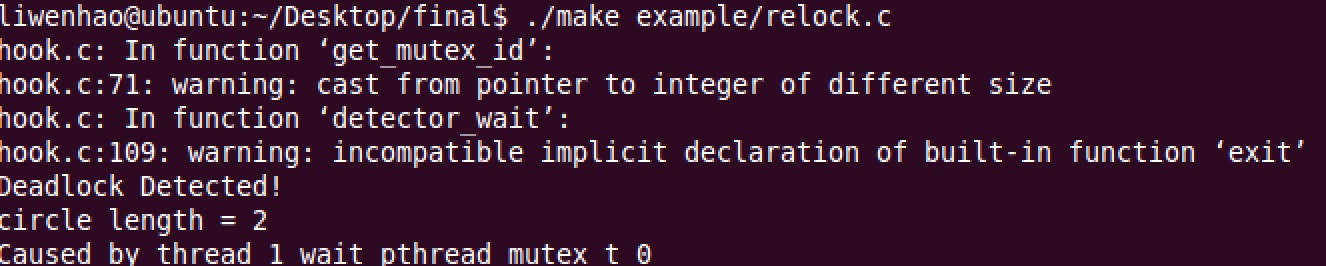
\includegraphics[scale=0.4]{example1.png}
\normalsize
\end{center}
\indent 我们发现了一个长度为2的环,这显然是进程因为进程1等待锁0,而锁0又已经被进程1所持有。

\subsection{MultiLock}
\indent 第二个例子,我们把经典的两个锁两个进程造成死锁扩展,变成2个进程,多个锁所造成的死锁,以下是程序的部分:
\begin{lstlisting}{language=C}

const int M = 20;
pthread_mutex_t level[20 + 1];

void *func_a() {
        int i, count = CNT;
        while (count--) {
        printf("a start %d\n", count);
        for (i = 0; i < M; i++) {
            printf("a want %d\n", i);
            pthread_mutex_lock(&level[i]);
        }
        puts("a");
        for (i = M - 1; i >= 0; i--) {
            pthread_mutex_unlock(&level[i]);
        }
        printf("a over %d\n", count);
    }
}

void *func_b() {
    int i, count = CNT;
    while (count--) {
        printf("b start %d\n", count);
        for (i = M - 1; i >= 0; i--) {
            printf("b want %d\n", i);
            pthread_mutex_lock(&level[i]);
        }
        puts("b");
        for (i = 0; i < M; i++) {
            pthread_mutex_unlock(&level[i]);
        }
        printf("b over %d\n", count);
    }
}

\end{lstlisting}
\indent 对于这种死锁,很显然,是因为a, b进程与c, d资源交叉需求与持有造成的死锁,死锁的环的长度应该为4。以下是程序输出的结果。
\begin{center}
\footnotesize
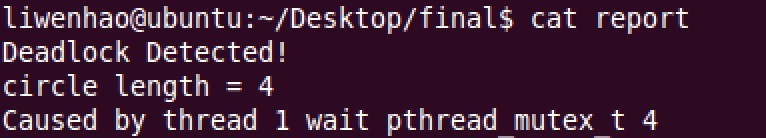
\includegraphics[scale=0.4]{example2.png}
\normalsize
\end{center}

\subsection{ProdAndCons}
\indent 这里测试的是最经典的消费者与生产者模型,由于代码很长,又特别经典,就不再贴上来了。由于模型过于经典,写法也是没有任何死锁的可能,经过我们程序的测试,的确没有产生死锁的结果。
\begin{center}
	\footnotesize
	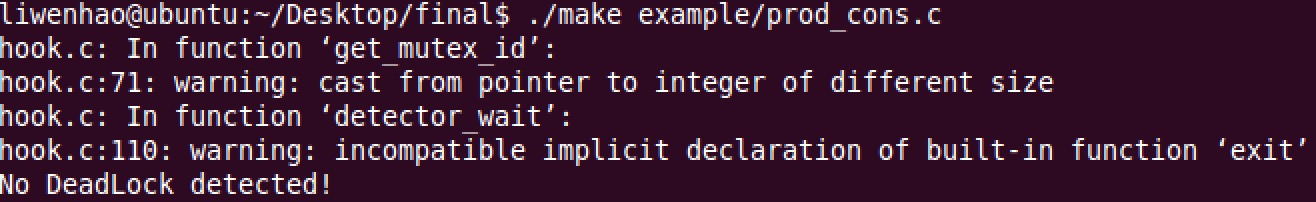
\includegraphics[scale=0.4]{example3.png}
	\normalsize
\end{center}

\subsection{WaitAndSignal}
\indent 为了测试我们实现的signal与wait造成的死锁,我们制造了这样的一个例子:
\begin{lstlisting}{language=C}
pthread_cond_t cond;
pthread_mutex_t s,b;
pthread_t aa,bb;

void *fa(void *argv) {
	pthread_mutex_lock(&s);
	pthread_mutex_lock(&b);
	printf("Done\n");
	pthread_cond_wait(&cond, &s);
	printf("Start?\n");
	pthread_mutex_unlock(&s);
	pthread_mutex_unlock(&b);
	pthread_exit(0);
}
void *fb(void *argv) {
	sleep(1);
	pthread_mutex_lock(&s);
	printf("Locked\n");
	pthread_cond_signal(&cond);
	printf("Sent\n");
	pthread_mutex_lock(&b);
	pthread_mutex_unlock(&s);
	pthread_mutex_unlock(&b);
	pthread_exit(0);
}
int main() {
	pthread_mutex_init(&s, 0);
	pthread_mutex_init(&b, 0);
	pthread_cond_init(&cond, 0);
	pthread_create(&aa, 0, fa, 0);
	pthread_create(&bb, 0, fb, 0);
	pthread_join(aa,0);
	pthread_join(bb,0);
	pthread_mutex_destroy(&s);
	pthread_mutex_destroy(&b);
	pthread_cond_destroy(&cond);
	return 0;
}

\end{lstlisting}
\indent 这样一个程序的死锁埋的有点深,在于在进程B signal了之后,进程A其实一直在等待自己的那把锁,所以我们需要hook signal函数,在signal的同时去进行相应的加边操作。

\begin{center}
\footnotesize
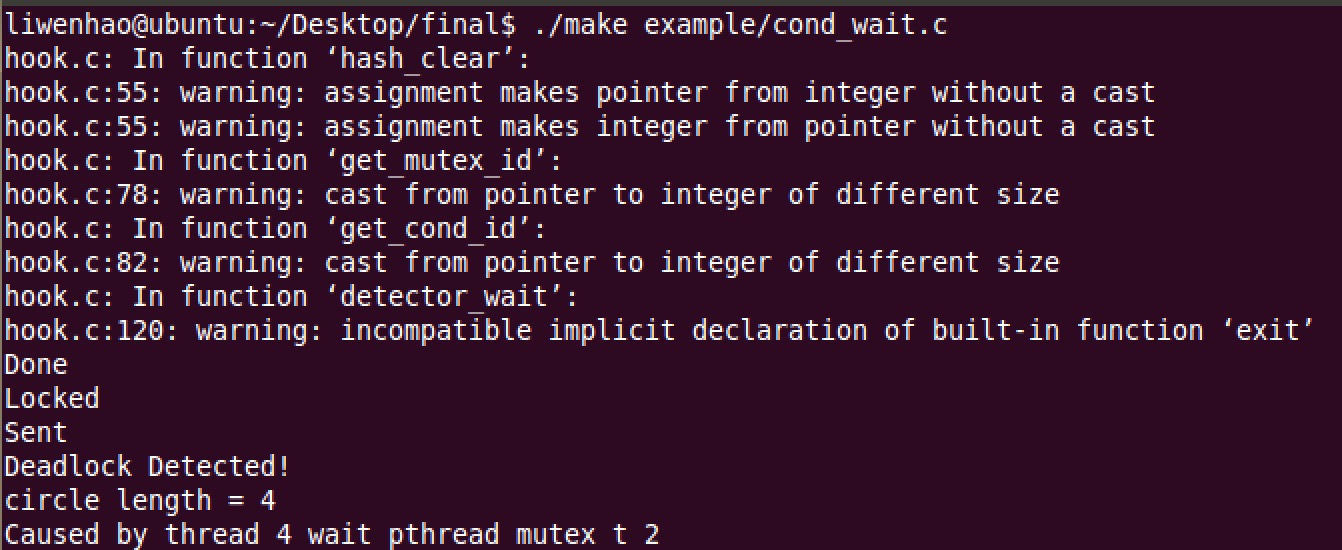
\includegraphics[scale=0.4]{example4.png}
\normalsize
\end{center}
\indent 可以发现,我们的程序很好地检测到了这一类的死锁。


\section{Thought and Conclusion}
\indent 这次的死锁检测Project是一次很有意思的实验,对于我们三个没有研究过linux源码的人来说,起步着实是一件很困难的事。在这之中,我们进行了很多无用的尝试,最后才得到我们的成果,我想在这里列举一点我们遇到的困难。
\begin{itemize}
	\item[1.] 如何使用Hook。\\
一开始我们是决定在内核级别使用Hook来得到更多的信息,而由于在内核态遇到的太多的困难导致我们不得不选择在用户态做。
	\item[2.] 哪些函数和死锁有关,线程库的源码。\\
为了不在我们自己的算法层面出现死锁的情况,我们不得不经过了很多的考究,包括我们Hook的各个函数之间的影响,这里想要做到没有错误也是需要很多的考究。
	\item[3.] 我们到底还可以做到什么。\\
为了能尽可能的检测到多的死锁,我们也思考了很多死锁的形式,其中一个就是signal信号的丢失。还有内核级别的死锁检测。甚至,关于死锁预防和死锁解除我们也了解了一些资料,但是这都是一些理论上的知识,要真的实现的确是不太可能。
\end{itemize}
\indent 我认为我们所做的尝试虽然很多都失败了,但是还是很有启发意义,每一次失败都能使我们对linux更深切的领悟。十分感谢这次做Project的机会,也谢谢大家一起的合作。


\section{Task Assignment}

\subsection{高宇}
\begin{itemize}
	\item[1.] 算法设计(包括算法中可能涉及到的死锁)。
	\item[2.] 程序正确性的检查。
	\item[3.] 撰写report。
\end{itemize}

\subsection{张家睿}
\begin{itemize}
	\item[1.] 内核态和用户态的Hook方法的研究。
	\item[2.] 设计Example
\end{itemize}

\subsection{李文昊}
\begin{itemize}
	\item[1.] 资料收集,对线程库的资料研究。
	\item[2.] 代码实现,debug。
\end{itemize}

\end{document}
